\section{Part A}
	
 \begin{itemize}
 \item
 On the congressional votes dataset given in "p1\_congress\_1984\_votes.csv", apply principal component analysis (PCA). Plot the cumulative variance explained by top $k$ principal components (with highest eigenvalues) as a function of $k$ (see \text{"example\_pca\_figure.png"}). How many principal components do you think are enough to sufficiently summarize the data (according to the explained variance)? 
 
 \item
 Next, project the data onto the first 3 principal components with highest eigenvalues. For each of the three principal component pairs (PC1-PC2, PC1-PC3, PC2-PC3), draw a scatter plot of congress members colored according to their party affiliations\\ (as given in "p1\_congress\_1984\_party\_affiliations.csv"). Which of the principal component pair separates the congress members best according to their party affiliations? Are the congress members with the same party affiliation seem to be clustered according to their votes on the congress?
\end{itemize}
 
-----\\

The PCA implementation and cumulative variance code are given below:

\begin{verbatim}
def congress_pca(data: np.ndarray, n_components: int = None) -> tuple:
    """
    Applies PCA to the congressional voting data.
    
    :param data: Feature matrix
    :type data: np.ndarray
    :param n_components: Number of components to keep
    :type n_components: int or None
    :returns: PCA model, transformed data, explained variance ratio
    :rtype: tuple
    """
    
    pca = PCA(n_components=n_components)
    data_pca = pca.fit_transform(data)
    explained_variance = pca.explained_variance_ratio_
    
    return pca, data_pca, explained_variance

def plot_cumulative_variance(explained_variance: np.ndarray, 
                            output_filename: str):
    """
    Plots cumulative variance explained by top k principal components.
    
    :param explained_variance: Array of explained variance ratios
    :type explained_variance: np.ndarray
    :param output_filename: Filename for output figure
    :type output_filename: str
    """
    cumulative_variance = np.cumsum(explained_variance)
    k_values = np.arange(1, len(cumulative_variance) + 1)
    
    sns.set_style("whitegrid")
    sns.set_palette("muted")
    plt.figure(figsize=(10, 6))
    
    plt.plot(k_values, cumulative_variance, marker='o', 
             linewidth=2, markersize=6, color='steelblue')
    
    plt.xlabel('Number of Principal Components (k)', fontsize=14, labelpad=15)
    plt.ylabel('Cumulative Variance Explained', fontsize=14, labelpad=15)
    plt.title('Cumulative Variance Explained by Top k Principal Components', 
             fontsize=16, pad=20)
    plt.grid(True, alpha=0.3)
    plt.xlim(0, len(k_values) + 0.5)
    plt.ylim(0, 1.05)
    
    plt.tight_layout()
    os.makedirs("../figures", exist_ok=True)
    plt.savefig(f"../figures/{output_filename}", bbox_inches='tight', dpi=300)
\end{verbatim}

\begin{center}
\textbf{Figure 1:} PCA and cumulative variance visualization implementation.
\end{center}

Figure 2 shows the cumulative variance explained over $ k $ principal components:

\begin{center}
  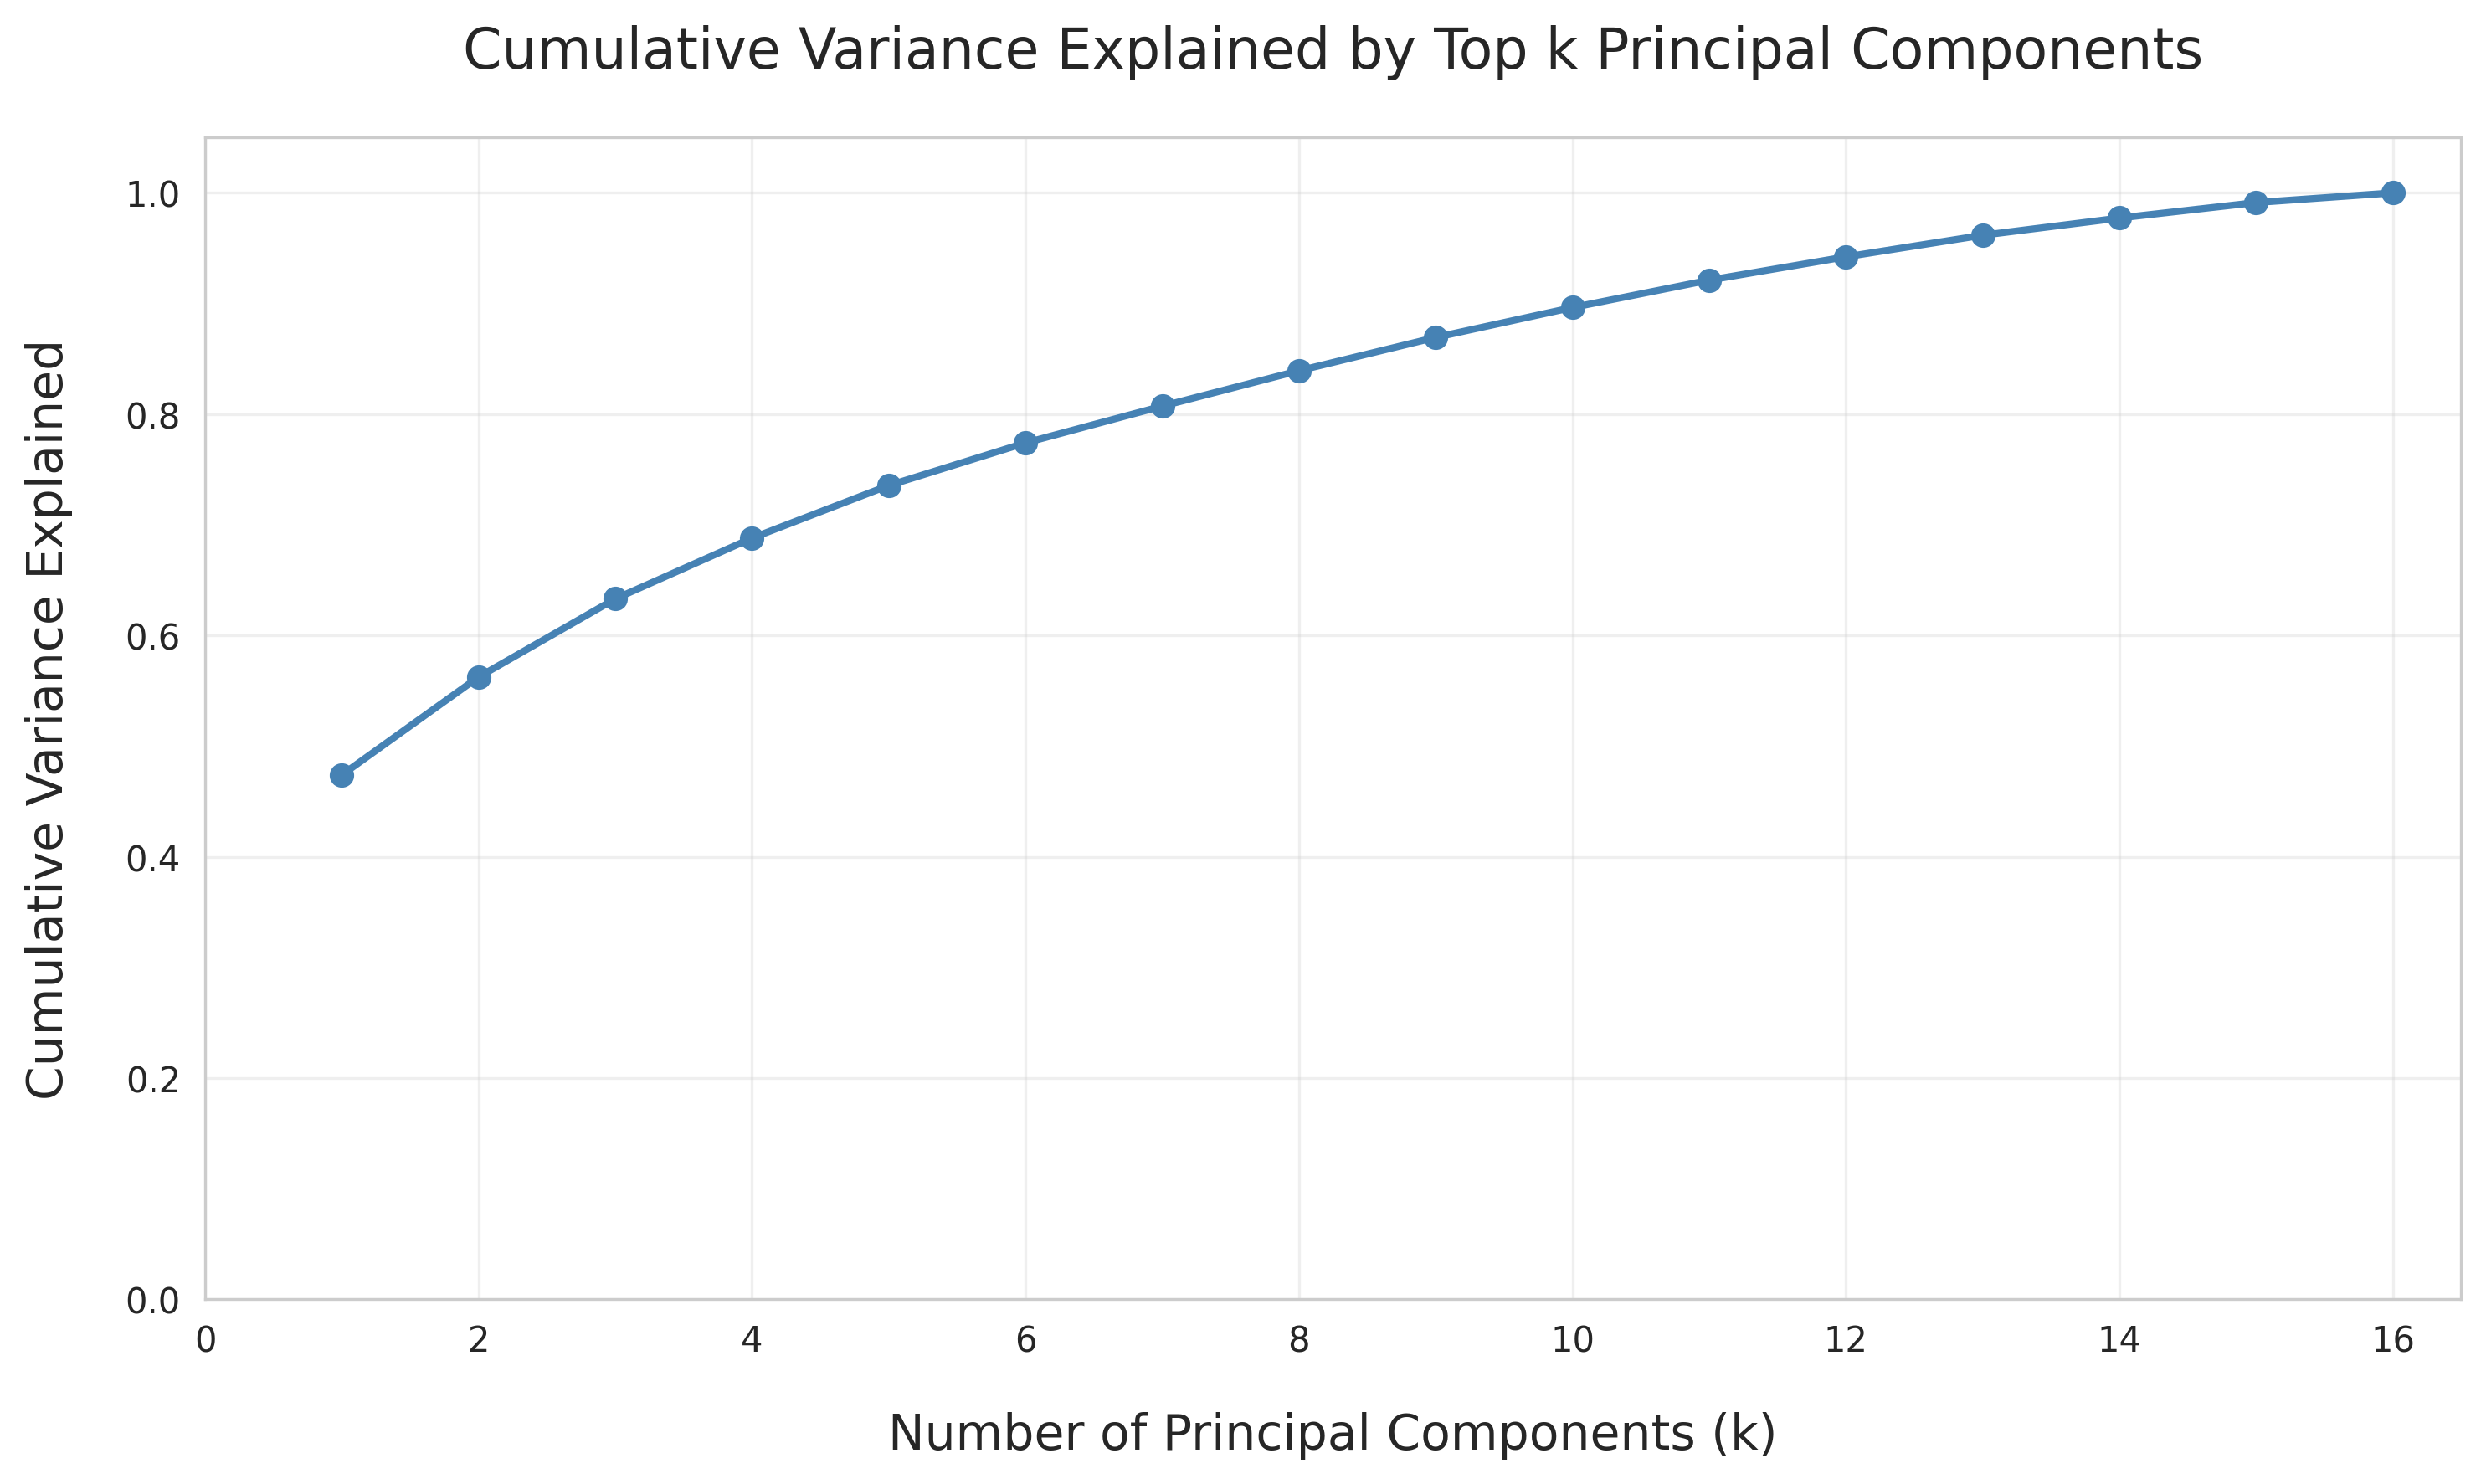
\includegraphics[width=0.95\textwidth]{figures/cumulative_variance_explained.png}
  
  \textbf{Figure 2:} Cumulative variance explained by top k principal components.
\end{center}

PC1 alone covers 47.4\% of the variance, and the first seven components together achieve 80\% with lesser value in additional components past that point. I would argue this number of the PCs well-represents the voting data while still maintaining value from the dimensionality reduction, though adding more up to around 10-11 components before returns are severely diminished could be appropriate for prioritizing fidelity/separation in the voting patterns. The separation produced by the PC projections are shown below alongside their corresponding implementation:

\begin{verbatim}
def plot_pc_scatter(data_pca: np.ndarray, party_labels: np.ndarray,
                   pc_x: int, pc_y: int, output_filename: str):
    """
    Plots scatter plot of two principal components colored by party.
    
    :param data_pca: pca-transformed data
    :type data_pca: np.ndarray
    :param party_labels: Party affiliation labels
    :type party_labels: np.ndarray
    :param pc_x: Index of PC for x-axis
    :type pc_x: int
    :param pc_y: Index of PC for y-axis
    :type pc_y: int
    :param output_filename: Filename for output figure
    :type output_filename: str
    """
    sns.set_style("whitegrid")
    sns.set_palette("muted")
    plt.figure(figsize=(10, 6))
    
    # Creates color mapping for parties
    unique_parties = np.unique(party_labels)
    colors = {'republican': 'red', 'democrat': 'blue'}
    
    for party in unique_parties:
        mask = party_labels == party
        party_lower = party.lower()
        color = colors.get(party_lower, 'gray')
        
        plt.scatter(data_pca[mask, pc_x], data_pca[mask, pc_y],
                   c=color, label=party.capitalize(), 
                   alpha=0.6, s=50, edgecolor='white', linewidth=0.5)
    
    plt.xlabel(f'PC{pc_x + 1}', fontsize=14, labelpad=15)
    plt.ylabel(f'PC{pc_y + 1}', fontsize=14, labelpad=15)
    plt.title(f'Congress Voting Separation on PC{pc_x + 1} vs PC{pc_y + 1}', 
             fontsize=16, pad=20)
    plt.legend(fontsize=11, loc='best')
    plt.grid(True, alpha=0.3)
    
    plt.tight_layout()
    os.makedirs("../figures", exist_ok=True)
    plt.savefig(f"../figures/{output_filename}", bbox_inches='tight', dpi=300)
\end{verbatim}

\begin{center}
\textbf{Figure 3:} PC projections scatter plot function.
\end{center}

\begin{center}
  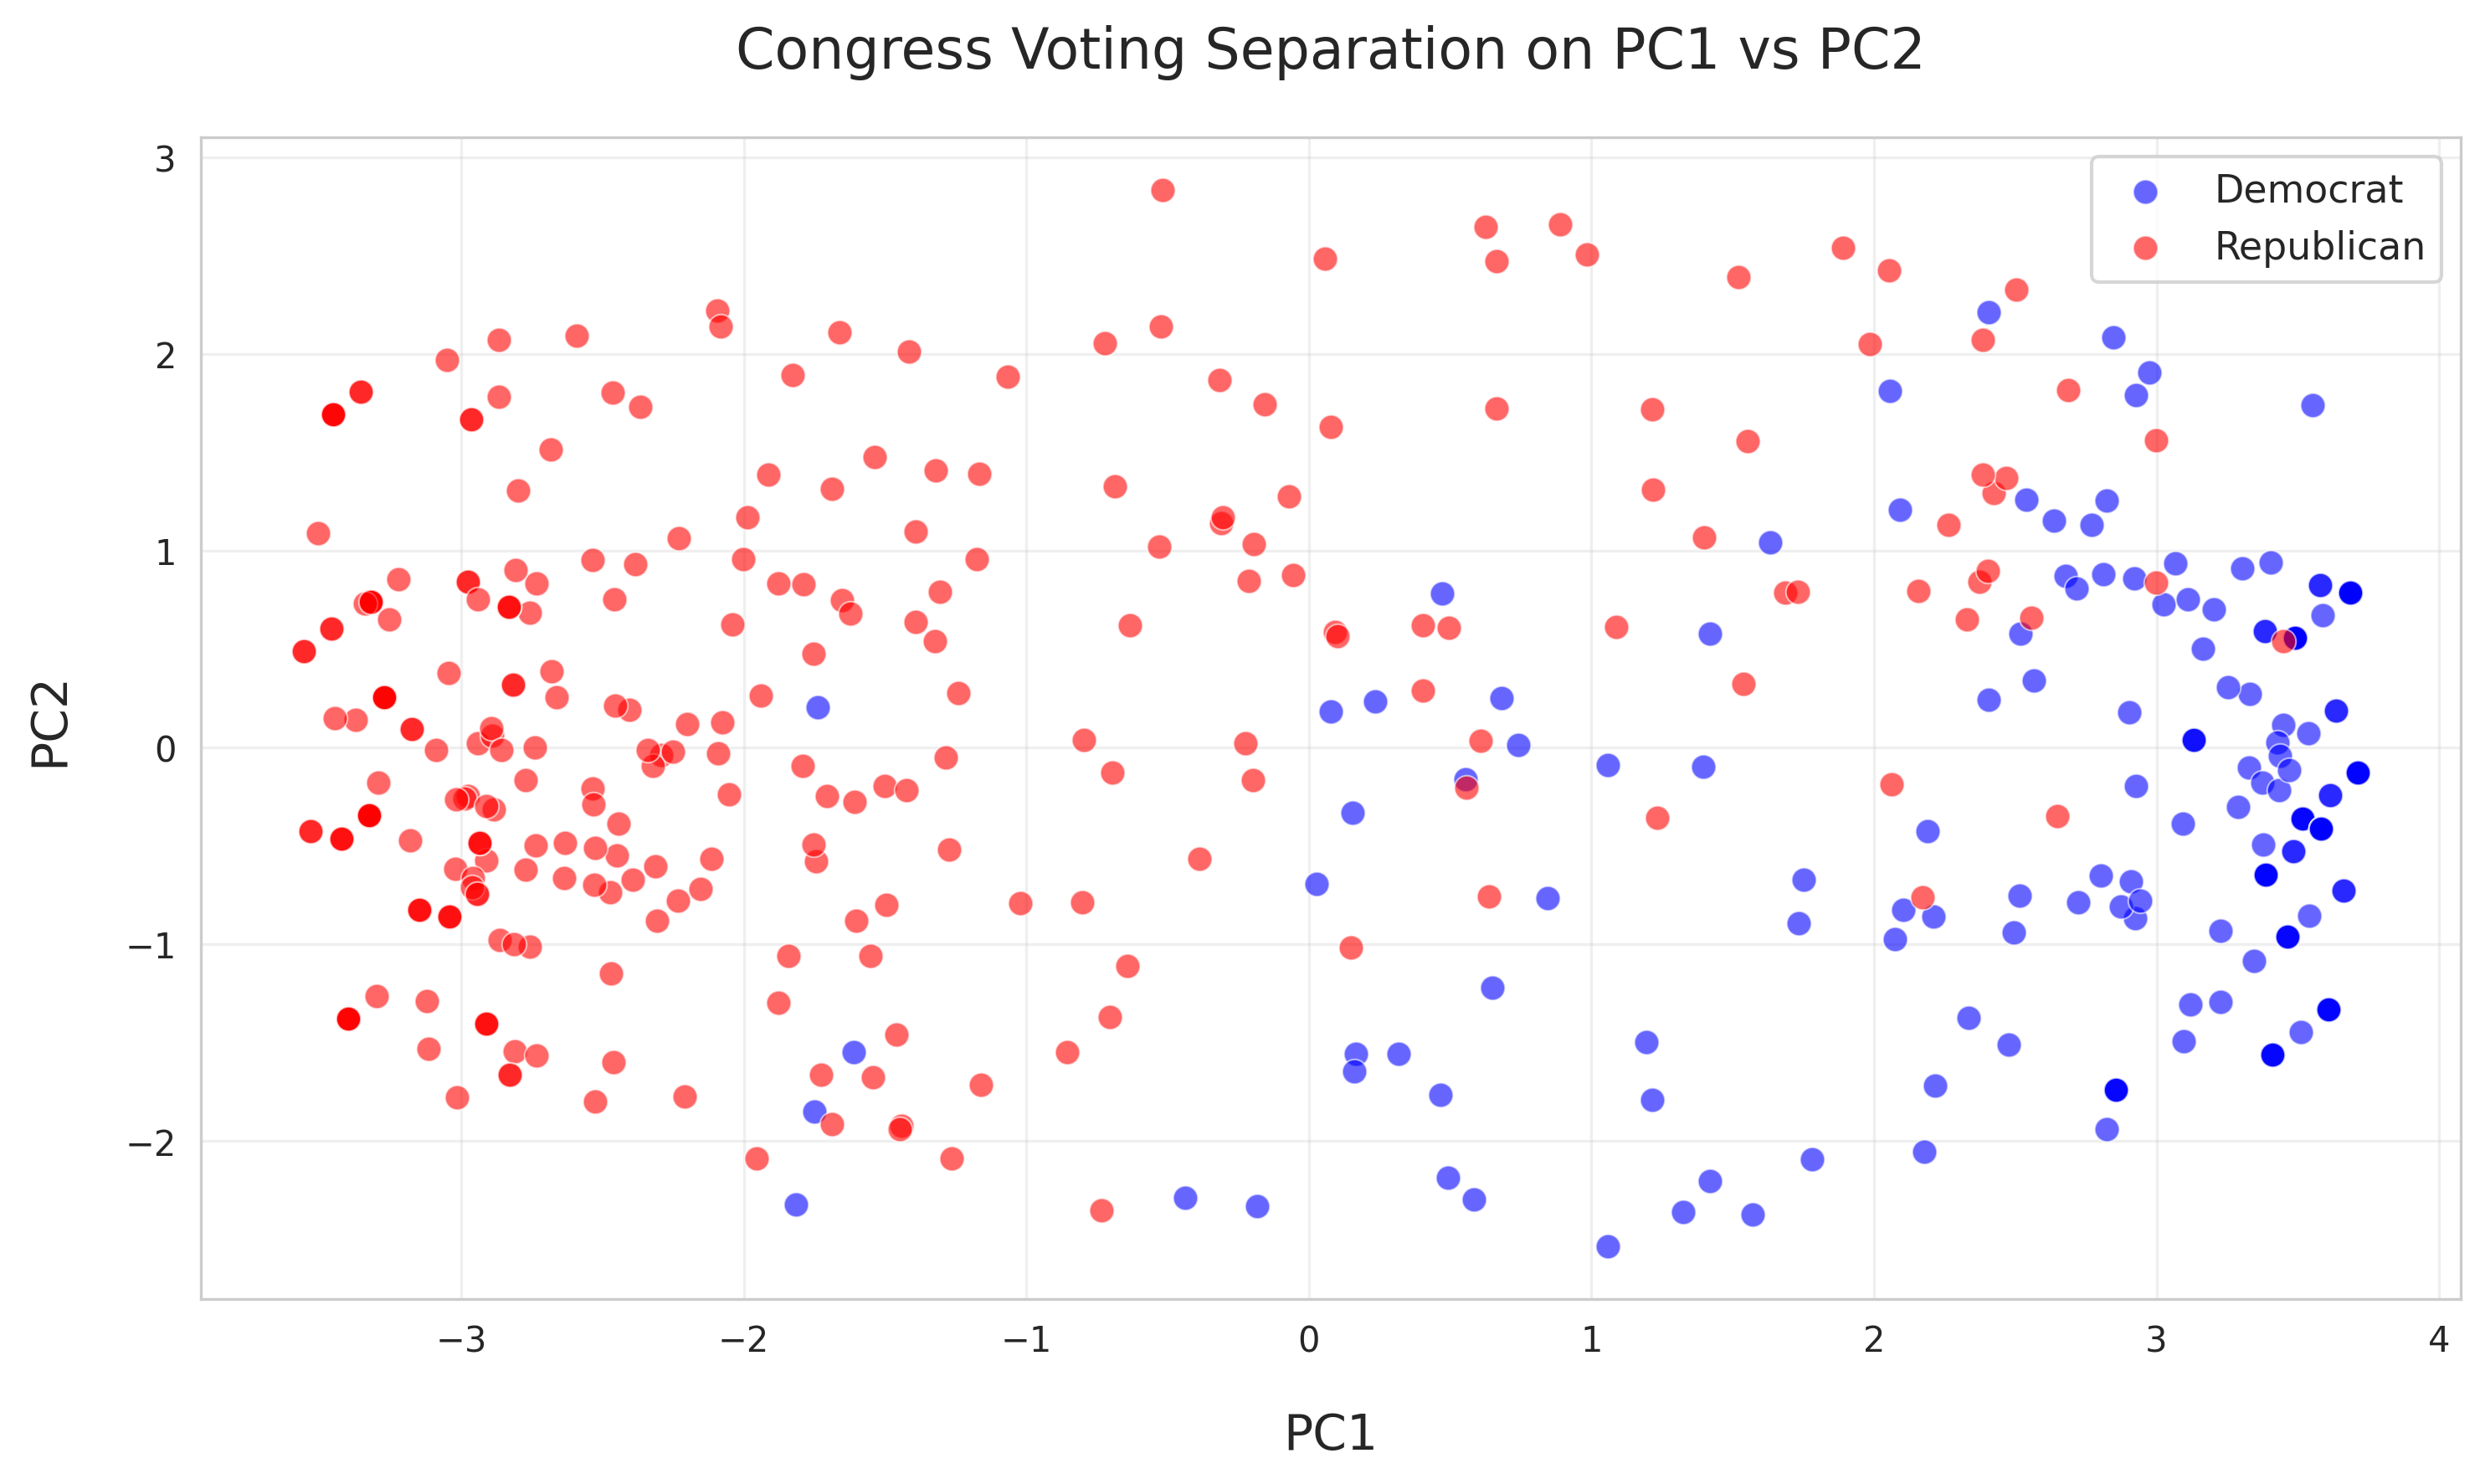
\includegraphics[width=0.95\textwidth]{figures/scatter_pc1_pc2.png}
  
  \textbf{Figure 4:} Congress members projected onto PC1 vs PC2, colored by party affiliation.
\end{center}

\begin{center}
  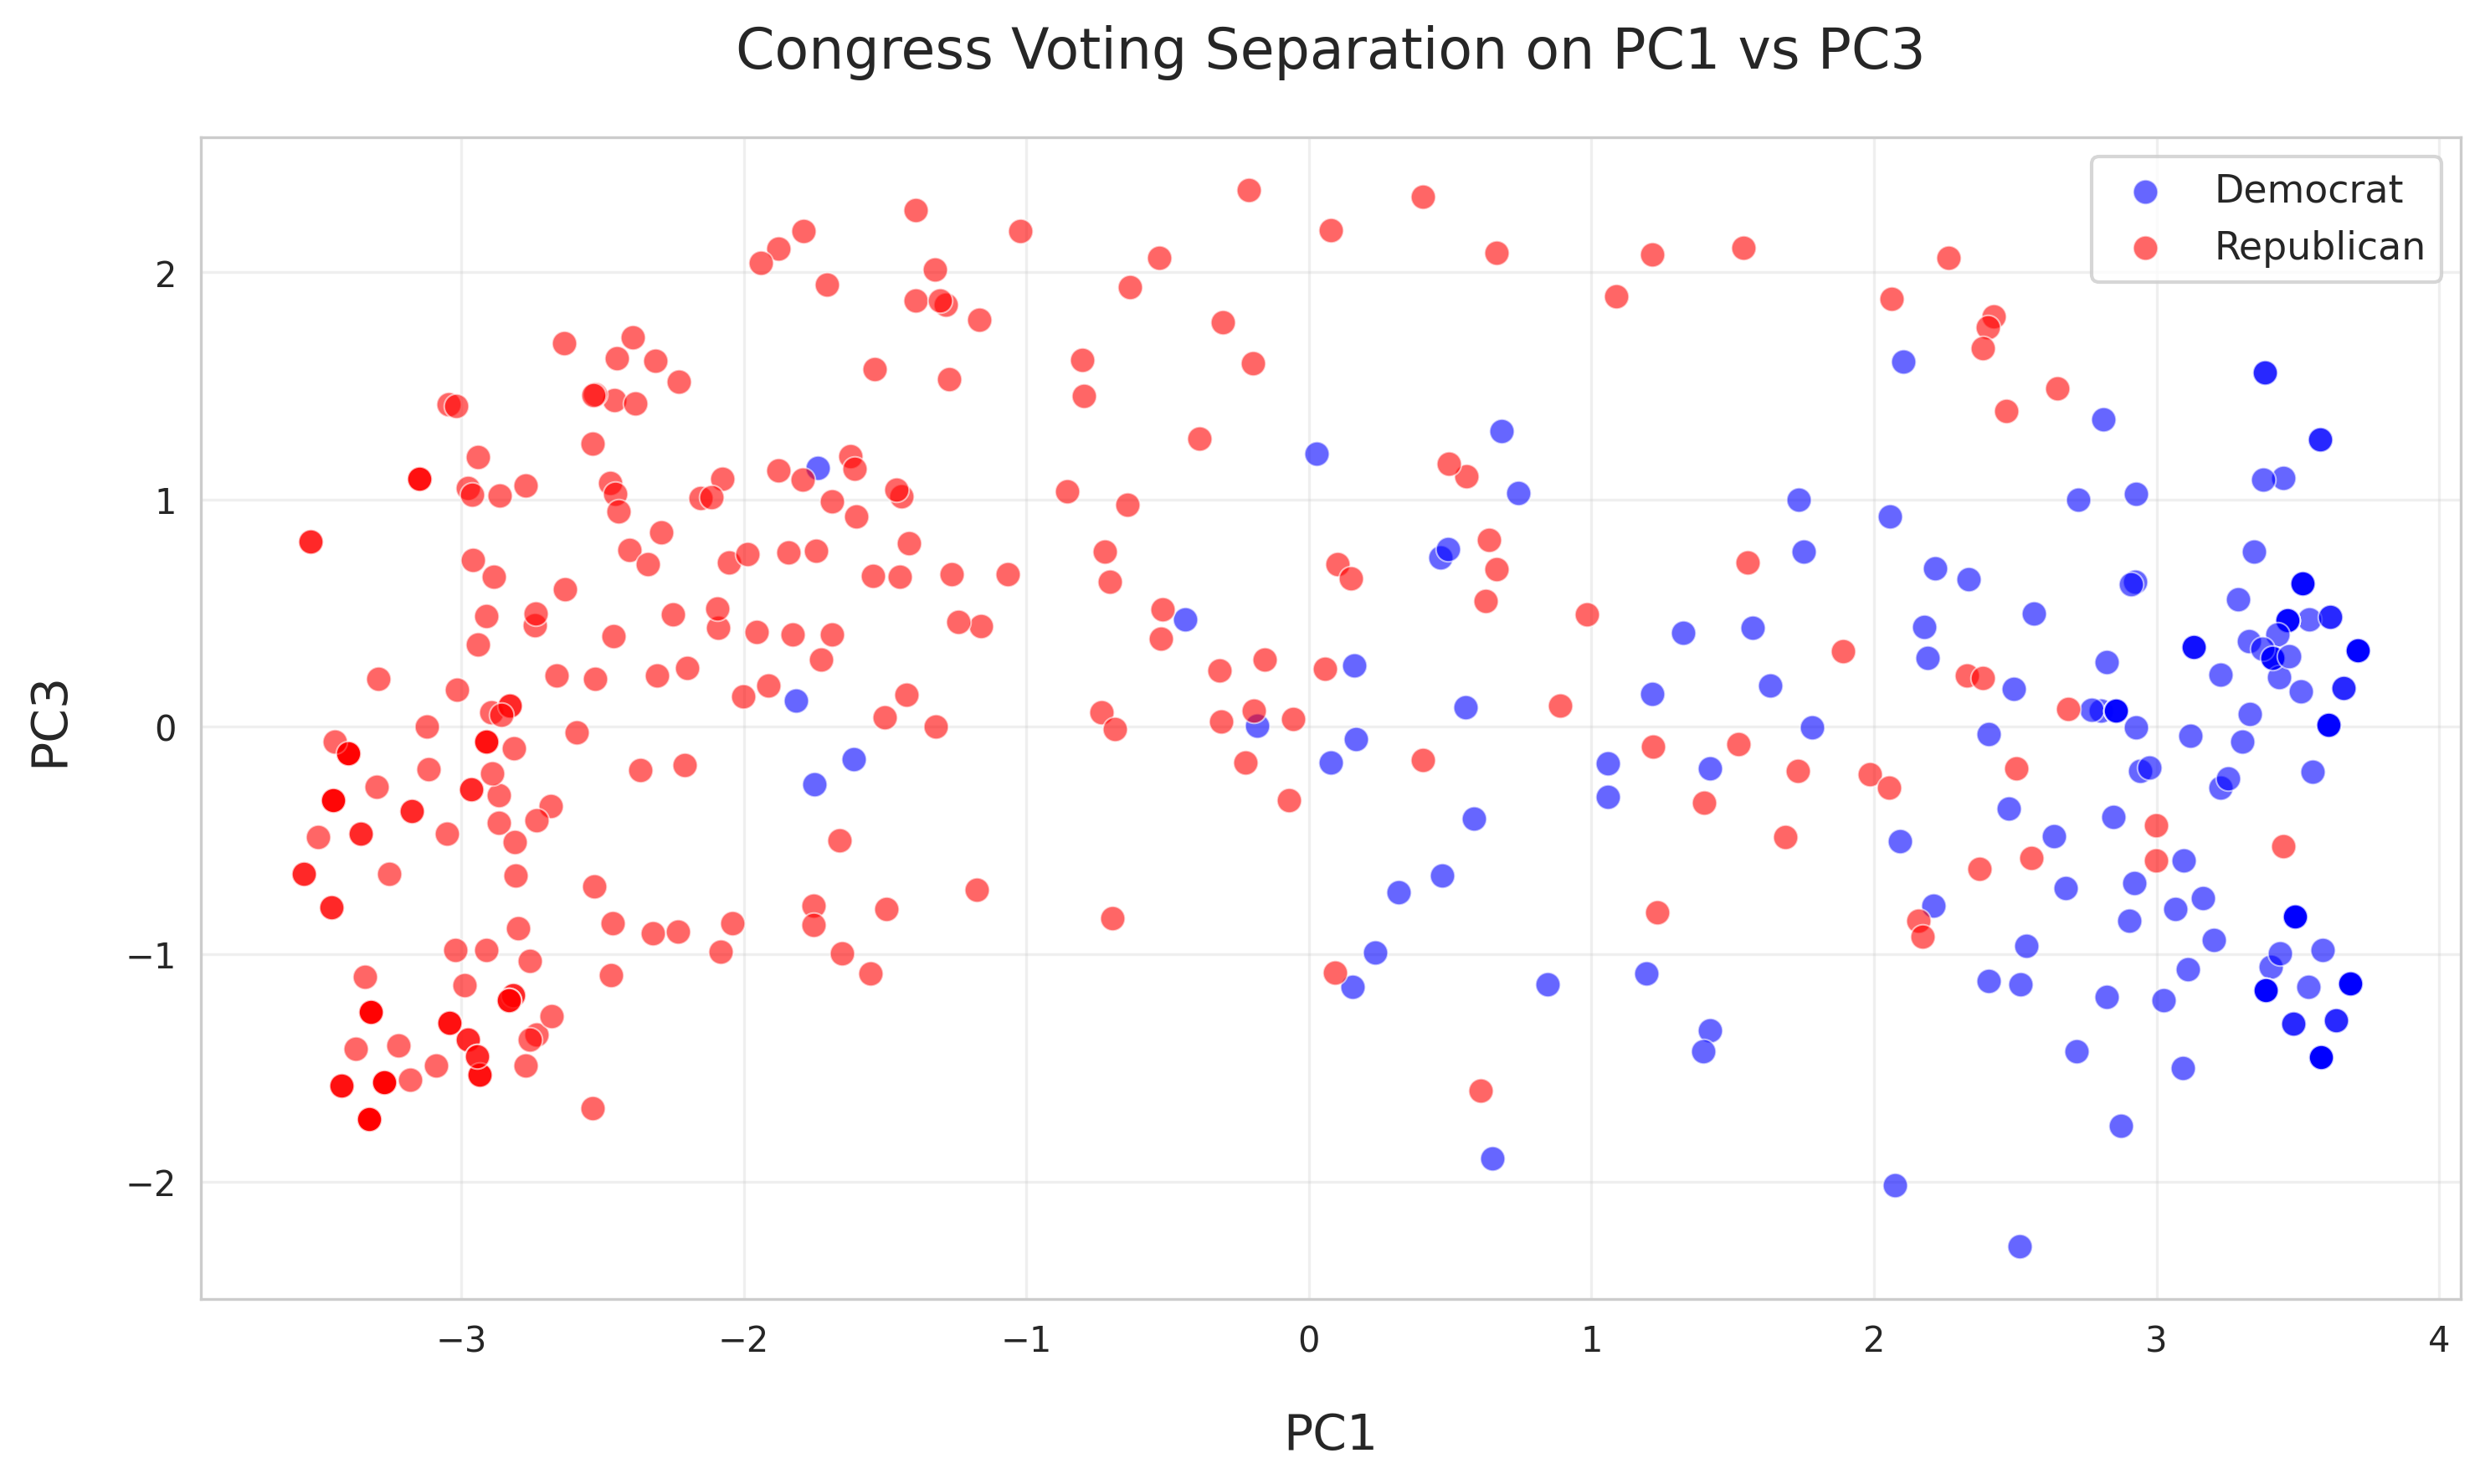
\includegraphics[width=0.95\textwidth]{figures/scatter_pc1_pc3.png}
  
  \textbf{Figure 5:} Congress members projected onto PC1 vs PC3, colored by party affiliation.
\end{center}

\begin{center}
  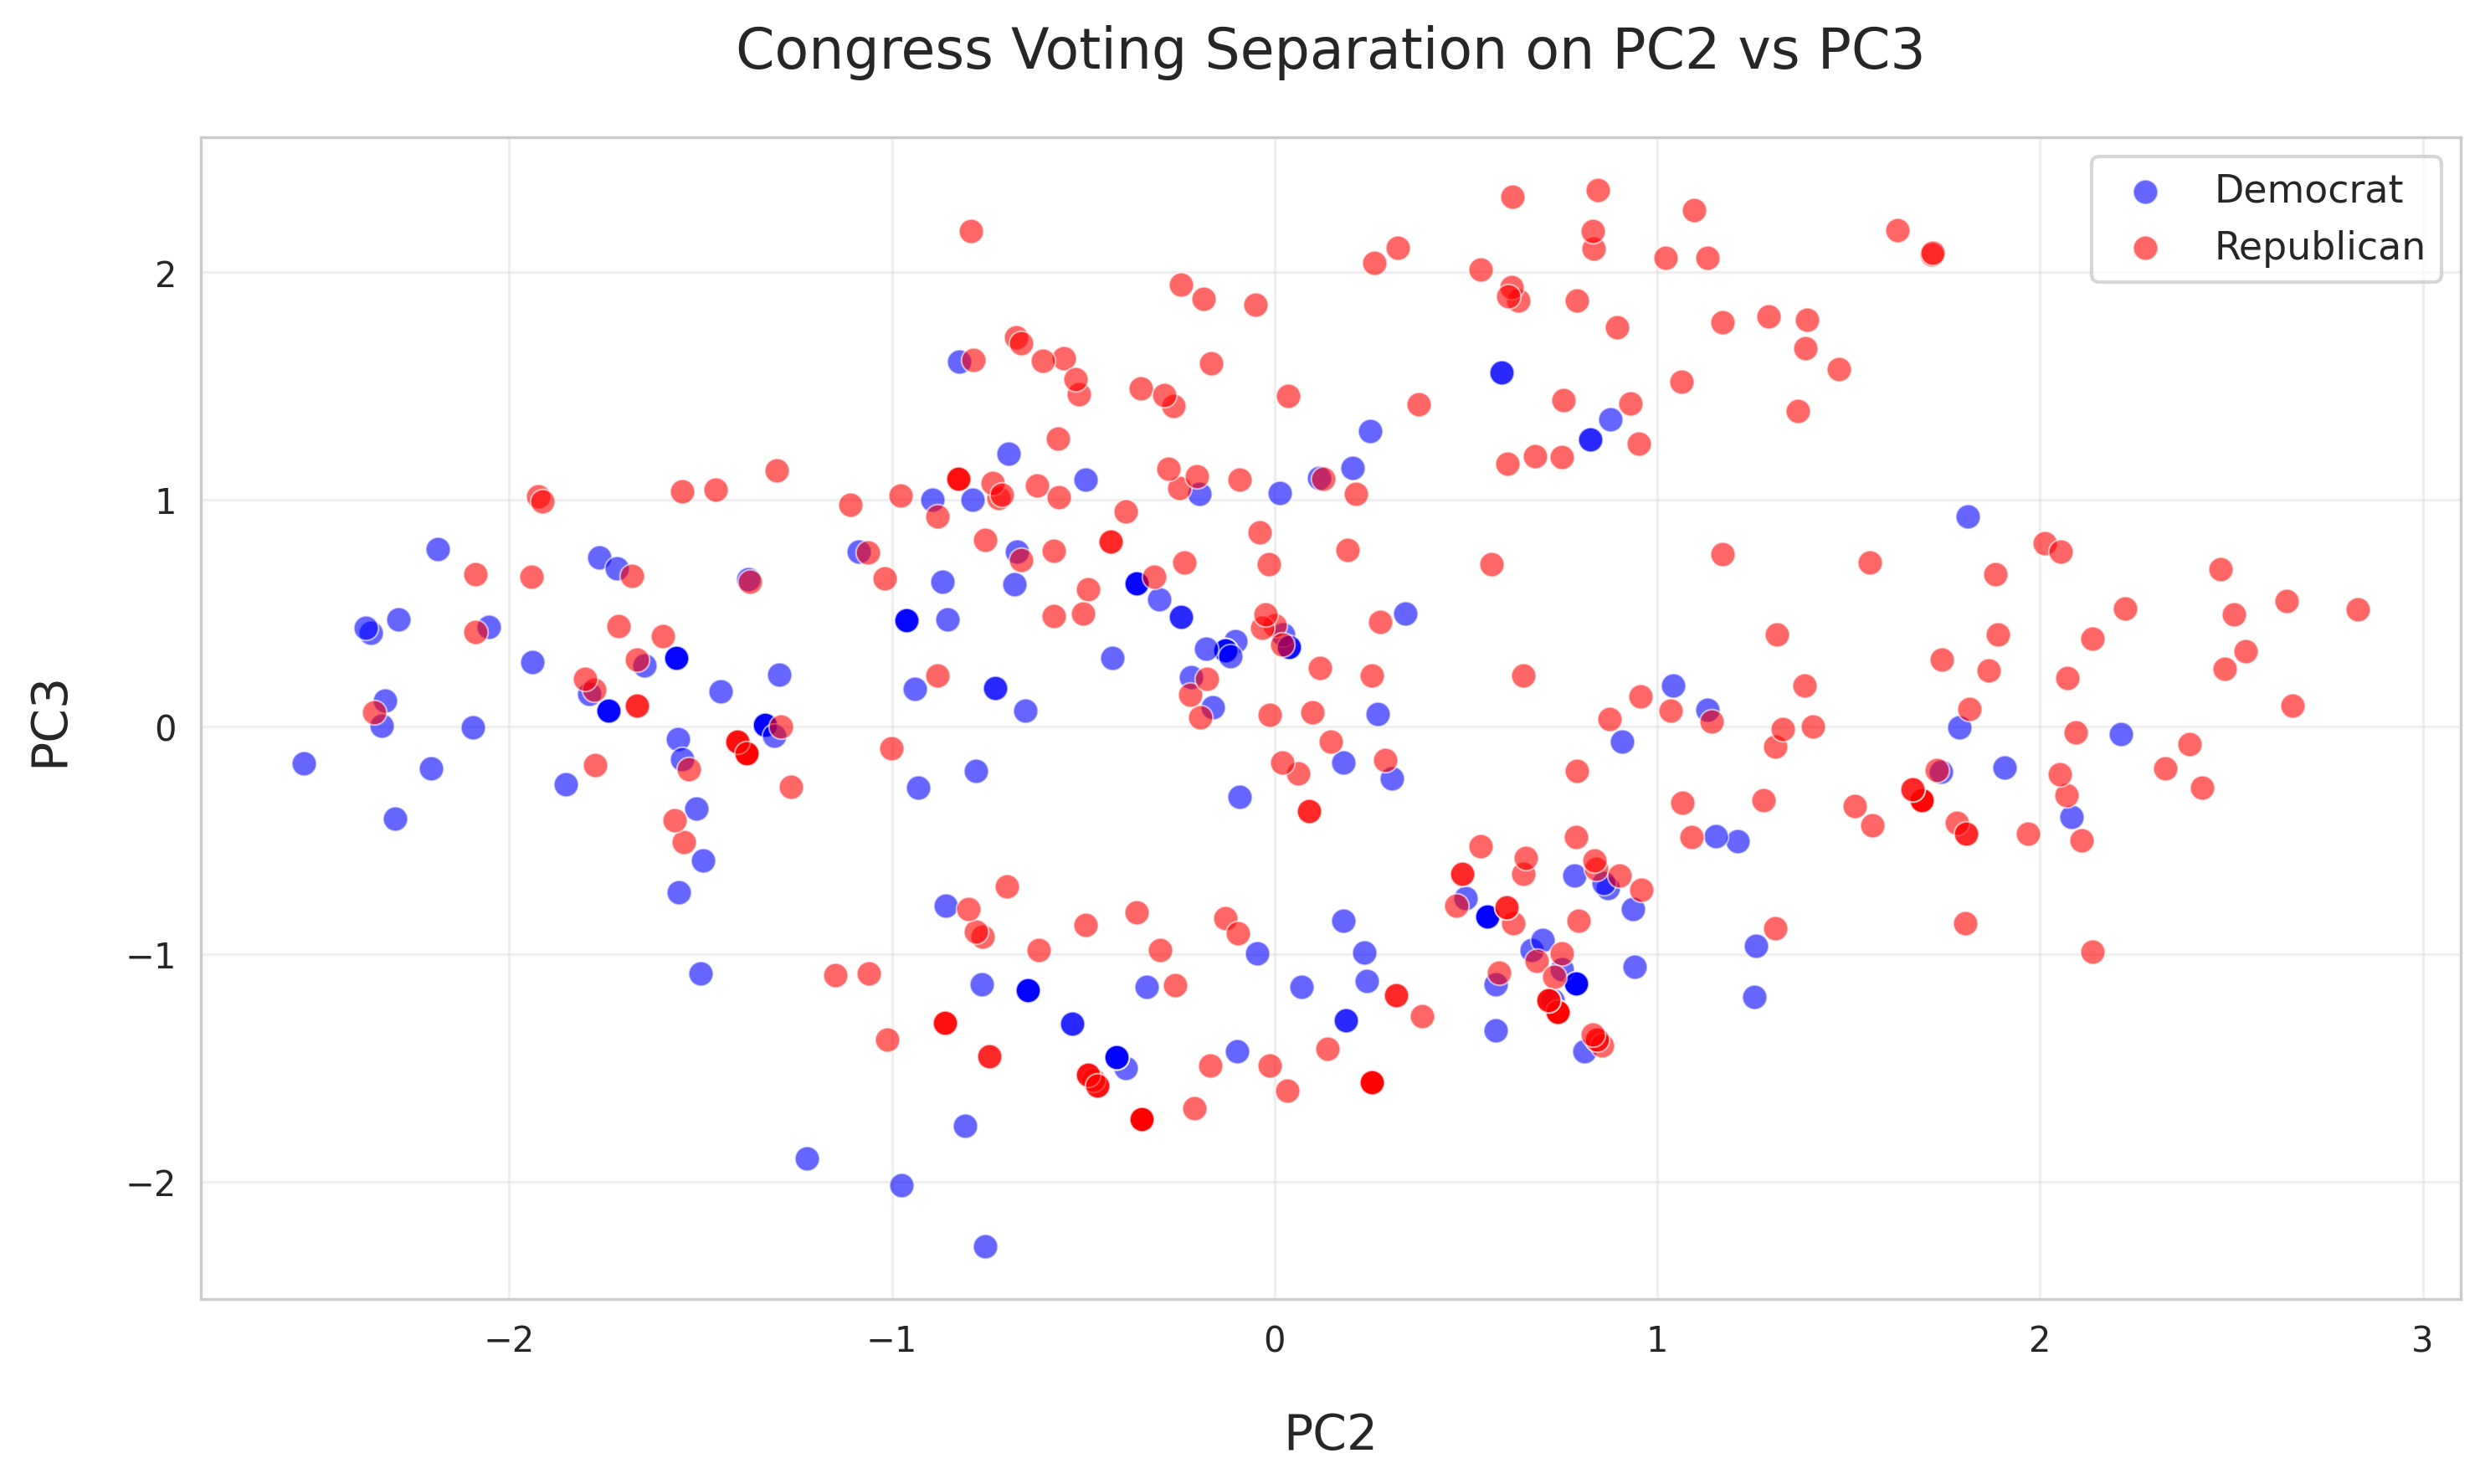
\includegraphics[width=0.95\textwidth]{figures/scatter_pc2_pc3.png}
  
  \textbf{Figure 6:} Congress members projected onto PC2 vs PC3, colored by party affiliation.
\end{center}

The PC1-PC2 projection produced the best separation of the congress members by political party. PC1-PC3 performs similar, but it is visually apparent that PC2 does marginally better to pull (R) members in the positive direction and (D) in the negative; PC2-PC3 shows much of the value lost from PC1, which as we saw largely dominates the cumulative variance. From the PC2-PC3 plot, we also get a better look at the better separation achieved by PC2 over PC3 more directly. As you would expect, the separation is immediately visually apparent along PC1, with (R) members on on the left and (D) on the right with an expected small number of moderate players floating in the middle and just a handful leaning toward the opposing party.\\

The congress members of the same political party do appear to cluster together in this plot based on their voting patterns, suggesting that party affiliation is a decent indicator of voting behavior on key congressional issues, with PC1 being a fairly suitable party line dimension, as it covers nearly half of all the variance.

\newpage
